\documentclass{sig-alternate}

\usepackage{booktabs}
\usepackage{amsmath}
\usepackage{amssymb}
\usepackage{algorithm}
\usepackage{algpseudocode}
\usepackage{hyperref}
\usepackage{microtype}
\usepackage[capitalise]{cleveref}
\usepackage{pgfgantt}
\usepackage{tikz}
\usetikzlibrary{shapes.geometric, arrows.meta, positioning, fit, backgrounds}

\makeatletter
\let\@copyrightspace\relax
\makeatother

\makeatletter
\renewcommand\section{\@startsection{section}{1}{\z@}%
    {-10\p@ \@plus -4\p@ \@minus -2\p@}%
    {16\p@}%
    {\baselineskip 14pt\secfnt\@ucheadtrue}}
\renewcommand\subsection{\@startsection{subsection}{2}{\z@}%
    {-8\p@ \@plus -2\p@ \@minus -\p@}%
    {12\p@}%
    {\secfnt}}
\renewcommand\subsubsection{\@startsection{subsubsection}{3}{\z@}%
    {-8\p@ \@plus -2\p@ \@minus -\p@}%
    {10\p@}%
    {\subsecfnt}}
\makeatother

\begin{document}

\conferenceinfo{ICS5200 Progress Report}{2025/2026, University of Malta}

\title{Uncertainty-Conditioned Reinforcement Learning\\ with Evidential Policy Networks\\ for Autonomous Systems}

\numberofauthors{1}
\author{
    \alignauthor Antonio Galdes\\
        \affaddr{University of Malta}\\
        \affaddr{Faculty of ICT}\\
        \email{antonio.galdes.22@um.edu.mt}
}
\maketitle

\begin{abstract}
Autonomous parking systems trained with reinforcement learning typically assume reliable localisation, yet sensor quality fluctuates unpredictably in practice. This report presents an uncertainty-conditioned reinforcement learning architecture that addresses this limitation through two complementary mechanisms. The first embeds six Extended Kalman Filter (EKF) posterior covariance elements (the three marginal standard deviations and three cross-covariance terms) directly into the policy observation vector. The second replaces the standard Gaussian actor head with a Normal-Inverse-Gamma (NIG) evidential output layer, yielding per-action epistemic and aleatoric uncertainty in a single forward pass. Together, these methods create an uncertainty-conditioned policy that is trained via Proximal Policy Optimisation (PPO) in the CARLA simulator under dynamically changing fix-states of the Real-Time Kinematic Global Navigation Satellite System (RTK-GNSS), which are represented by a discrete-time Markov chain. Moreover, a $2 \times 2$ factorial ablation study is proposed to isolate the contribution of each uncertainty layer to collision avoidance under degraded localisation.
\end{abstract}

% \category{I.2.6}{Artificial Intelligence}{Learning}[connectionism and neural nets]
% \category{I.2.9}{Artificial Intelligence}{Robotics}[autonomous vehicles]
% \terms{Algorithms, Design, Reliability}
\keywords{Reinforcement learning, evidential deep learning, uncertainty quantification, autonomous parking, localisation uncertainty, Extended Kalman Filter}

\section{Introduction}
\label{sec:introduction}

In the autonomous-driving sector, reinforcement learning (RL) is frequently utilised for vehicle control~\cite{yurtsever2020survey}, usually on the assumption that the localisation system delivers accurate pose estimates throughout operation. In practice, RTK-GNSS accuracy deteriorates from centimetre to metre level depending on satellite visibility and atmospheric conditions. Additionally, automotive functional safety standards like ISO~26262~\cite{iso26262} prohibit the deployment of a parking system that collides with obstacles when localisation quality deteriorates. As a result, policies that were trained without considering the quality of localisation are unable to change when circumstances require it.

This problem is influenced by two different kinds of uncertainty. According to Kendall and Gal~\cite{kendall2017uncertainties}, aleatoric uncertainty captures irreducible noise in the environment and persists regardless of data quantity~\cite{charpentier2022disentangling}, whereas epistemic uncertainty reflects the model's ignorance of unfamiliar states and can be reduced with additional training data. Both these types of uncertainty can be quantified through evidential deep learning (EDL), a framework that has been applied to the value-estimation component of actor-critic architectures~\cite{akgul2025eppo}, to perception modules feeding model predictive controllers that optimise a finite-horizon action sequence at each step~\cite{ham2025dro} and to value-based discrete-action agents~\cite{stutts2024ceqr}.

Conditioning policies on uncertainty has also shown promise outside the EDL framework: uncertainty has been shown to provide a reliable signal for guiding agents in active exploration~\cite{placed2020active}, and localisation uncertainty alone can guide policy behaviour without evidential outputs~\cite{puthumanaillam2025guided}. Nevertheless, neither the actor of a continuous-action policy-gradient agent nor the raw Extended Kalman Filter (EKF) covariance elements have been provided as RL observation dimensions for vehicle control. The central question is whether incorporating localisation uncertainty, through pose covariance observation, evidential policy outputs, or both, yields measurably safer behaviour under degraded conditions.

The proposed system addresses this gap by placing an evidential NIG head on a continuous-action policy-gradient actor and feeding the EKF posterior covariance as an observation input. It will be evaluated on an outdoor parking task in the CARLA driving simulator~\cite{dosovitskiy2017carla} under dynamically changing GNSS quality.

\section{Aims and Objectives}
\label{sec:aims}

This study aims to create and assess an uncertainty-conditioned RL architecture that enables an autonomous parking agent to degrade gracefully under declining localisation quality, with the following objectives:

\begin{enumerate}
    \item Implement an EKF-based localisation pipeline within CARLA that fuses RTK-GNSS and Inertial Measurement Unit (IMU) data via the \texttt{robot\_localization} ROS~2 package~\cite{moore2014ekf} and produce a posterior covariance matrix reflecting sensor degradation. Correct operation will be assessed by verifying that steady-state covariance magnitude, averaged over repeated trials, increases monotonically in expectation across the four RTK fix-state tiers.
    \item Develop an evidential Proximal Policy Optimisation (PPO) algorithm~\cite{schulman2017ppo} in which the actor network outputs Normal-Inverse-Gamma (NIG) distributions over continuous actions~\cite{amini2020deep}, enabling single-pass quantification of epistemic and aleatoric uncertainty. The decomposition will be assessed by comparing uncertainty outputs across in-distribution and out-of-distribution conditions.
    \item Conduct a $2 \times 2$ ablation study comparing the full method against baselines lacking one or both uncertainty layers, measuring success rate and collision rate under both nominal and degraded GNSS conditions to isolate the contribution of each uncertainty layer.
\end{enumerate}

\section{Background and Literature Review}
\label{sec:background}

\subsection{Reinforcement Learning for Vehicle Control}

The Markov Decision Process (MDP) for sequential decision-making is defined by a tuple $(\mathcal{S}, \mathcal{A}, P, R, \gamma)$, where $\mathcal{S}$ is the state space, $\mathcal{A}$ the action space, $P$ the transition function, $R$ the reward function and $\gamma \in [0,1)$ the discount factor~\cite{sutton2018rl, thrun2005probabilistic}. At each time step $t$, the agent observes state $s_t \in \mathcal{S}$, selects action $a_t \in \mathcal{A}$, receives scalar reward $r_t$ and transitions to successor state $s_{t+1}$. A policy $\pi_\theta(a|s)$ then maps states to action distributions, parameterised by neural network weights $\theta$, and the objective is to determine $\theta$ such that the expected discounted return $\mathbb{E}[\sum_{t=0}^{\infty} \gamma^t r_t]$ is maximised. 

Policy gradient approaches use gradient ascent to optimise $\theta$ on this objective, but uncontrolled updates might result in unfavourable policy changes. This is reduced by PPO~\cite{schulman2017ppo}, which uses a clipped surrogate target to limit the scope of policy updates:

\begin{equation}
    L^{\text{CLIP}}(\theta) = \hat{\mathbb{E}}_t \left[ \min \left( r_t(\theta) \hat{A}_t, \; \text{clip}(r_t(\theta), 1{-}\epsilon, 1{+}\epsilon) \hat{A}_t \right) \right]
    \label{eq:ppo}
\end{equation}

\noindent where $r_t(\theta) = \pi_\theta(a_t|s_t) / \pi_{\theta_{\text{old}}}(a_t|s_t)$ denotes the probability ratio and $\hat{A}_t$ is the advantage estimate. This estimate is obtained via Generalised Advantage Estimation (GAE), which interpolates between single-step temporal-difference bootstraps and full-episode Monte Carlo return estimates using a trace-decay parameter $\lambda$~\cite{schulman2015gae}.

The complete training objective has three terms. The clipped surrogate from~\cref{eq:ppo} optimises the actor, an entropy bonus~\cite{mnih2016a3c} discourages premature convergence to a deterministic policy, and a value function loss~\cite{schulman2017ppo} trains the critic to produce advantage estimates on which the actor depends. This loss is defined as the squared residual between the critic's state-value estimate $V_\theta(s_t)$ and the empirical return $\hat{R}_t$:
\begin{equation}
    L^{\text{VF}}(\theta) = \left( V_\theta(s_t) - \hat{R}_t \right)^2.
\label{eq:vf_loss}
\end{equation}

\noindent Minimising this loss regresses the critic toward observed returns, providing the advantage estimates that drive the clipped policy objective.

PPO improves data efficiency over single-pass policy gradient approaches by gathering transitions across a fixed-length rollout, dividing them into mini-batches, and executing several gradient update epochs per rollout~\cite{schulman2017ppo}. In practice, training stability is further reinforced by two complementary measures: monitoring approximate KL divergence as a diagnostic early-stopping signal, and normalising observations via running statistics when input dimensions span different scales~\cite{raffin2021sb3}. These on-policy rollout properties make PPO a natural fit for the proposed system, as the clipped surrogate keeps policy stability and uncertainty quantification as separate concerns.

\subsection{Evidential Deep Learning}

Instead of learning point estimates, evidential deep learning sets a prior over the likelihood parameters. For regression, the target $y$ is modelled as being drawn from a Gaussian likelihood $\mathcal{N}(\mu, \sigma^2)$, and an NIG prior is imposed jointly over the unknown mean $\mu$ and variance $\sigma^2$~\cite{amini2020deep}. For each output dimension, the network produces four parameters $(\gamma, \nu, \alpha, \beta)$, where $\gamma$ is the predicted mean of $\mu$, $\nu > 0$ is the pseudo-observation count controlling the posterior concentration over $\mu$, and $\alpha > 1$, $\beta > 0$ parameterise the inverse-gamma prior over the observation variance $\sigma^2$. Two uncertainty types are then obtained in closed form:

\begin{equation}
    \sigma^2_{\text{alea}} = \frac{\beta}{\alpha - 1}, \qquad
    \sigma^2_{\text{epi}} = \frac{\beta}{\nu(\alpha - 1)}.
    \label{eq:nig_uncertainty}
\end{equation}

\noindent The aleatoric term is irreducible, whilst the epistemic term quantifies model uncertainty over $\gamma$ and shrinks as $\nu$ grows with evidence~\cite{kendall2017uncertainties}.

When evidential deep learning was first developed for classification~\cite{sensoy2018evidential}, it used a Dirichlet prior over class probabilities instead of generating point estimates. The framework was later extended to continuous regression through the NIG formulation~\cite{amini2020deep}, with the resulting uncertainty decomposition given in~\cref{eq:nig_uncertainty}. Since then, a gradient suppression effect has been discovered~\cite{oh2022improving}. As epistemic uncertainty grows, the gradient of the supervised evidential loss with respect to the predictive mean diminishes, causing the network to express uncertainty rather than refine its predictions. This problem is made worse in reinforcement learning, when the supervised penalty term is ill-defined due to the lack of ground-truth action targets. To address this, the proposed formulation is to add a prior-anchoring regularisation, which substitutes a limited log-penalty anchored to the NIG hyperprior for the supervised penalty.

Within reinforcement learning, evidential methods have so far been applied to the critic rather than the actor. Akg\"{u}l et al.~\cite{akgul2025eppo} address the non-stationarity of the target value distribution by placing an NIG evidential prior on the value function $V(s)$, whilst the actor retains a standard Gaussian policy. Stutts et al.~\cite{stutts2024ceqr} extend this to discrete-action contexts, pairing evidential Q-value estimation with quantile calibration to produce sample-free global uncertainty estimates. Beyond policy-gradient settings, a distinct line of work couples evidential uncertainty with an optimisation-based controller rather than a learnt policy~\cite{ham2025dro}, applying NIG-parameterised evidential deep learning under distributionally robust Model Predictive Control (MPC) constraints within CARLA.

In contrast to these single-pass evidential approaches, ensemble-based alternatives~\cite{lakshminarayanan2017ensembles} require multiple forward passes to obtain uncertainty estimates. In the MuJoCo simulator~\cite{todorov2012mujoco}, robustness in novel scenarios can be improved by conditioning the policy on ensemble disagreement~\cite{kim2022unicon}. In the autonomous driving domain, the Ensemble Quantile Networks method~\cite{hoel2023ensemble} combines per-quantile value distributions with independently initialised ensemble members to separately estimate aleatoric and epistemic uncertainty. The epistemic signal is then used to withhold decisions when out-of-distribution situations are encountered, eliminating most collisions outside the training distribution. Monte Carlo Dropout~\cite{gal2016dropout} reduces this to a single model but still requires several stochastic passes at inference time. The proposed single NIG forward pass avoids all of these overheads, generating both types of uncertainty concurrently and making it well-suited to control policies operating at high frequencies with low inference latency.

\subsection{Extended Kalman Filter Localisation}

The Kalman Filter (KF) is an optimal recursive Bayesian estimator for linear systems subject to Gaussian noise, propagating a Gaussian belief over the state through alternating prediction and update steps~\cite{thrun2005probabilistic}. Vehicle motion models however, are inherently nonlinear making the KF inapplicable. The EKF overcomes this by linearising the motion and measurement models via first-order Taylor expansion, substituting system matrices with their Jacobians at the current state estimate.

The EKF provides a principled means of fusing heterogeneous sensors such as GNSS and IMU into a continuous, covariance-bounded pose estimate, maintaining a Gaussian belief over the vehicle state $\mathbf{x}_t = [x, y, \psi]^\top$, where $x$ and $y$ are the planar position coordinates and $\psi$ is the heading angle (the full \texttt{robot\_localization} state also includes linear and angular velocities, but the planar pose subspace suffices to define the $3 \times 3$ covariance structure used here). The prediction step inflates the covariance according to process noise $\mathbf{Q}$:

\begin{equation}
    \mathbf{P}_{t|t-1} = \mathbf{F}_t \mathbf{P}_{t-1|t-1} \mathbf{F}_t^\top + \mathbf{Q}.
    \label{eq:ekf_predict}
\end{equation}

\noindent where $\mathbf{F}_t$ is the state transition Jacobian, $\mathbf{P}_{t-1|t-1}$ is the posterior covariance from the previous step and $\mathbf{Q}$ is the process noise covariance. The update step then incorporates a measurement with noise covariance $\mathbf{R}$:

\begin{equation}
    \mathbf{P}_{t|t} = (\mathbf{I} - \mathbf{K}_t \mathbf{H}_t) \mathbf{P}_{t|t-1}.
    \label{eq:ekf_update}
\end{equation}

\noindent where $\mathbf{K}_t$ is the Kalman gain, $\mathbf{H}_t$ is the measurement Jacobian and $\mathbf{I}$ is the identity matrix. The covariance $\mathbf{P}_{t|t}$ therefore grows between GNSS fixes and collapses upon each arriving measurement, producing a characteristic sawtooth profile. This time-varying posterior covariance is published alongside the pose estimate at each filter step by the \texttt{robot\_localization} package~\cite{moore2014ekf}, originally described for ROS~1 and subsequently ported to ROS~2, making it accessible to downstream components that condition on localisation uncertainty. The informativeness of this covariance signal is sensitive to process noise configuration, however, as Kovacs et al.~\cite{kovacs2025covariance} demonstrated, misconfigured process noise significantly degrades EKF localisation accuracy. Therefore, establishing careful noise parameterisation is a prerequisite for reliable covariance estimation.

\subsection{Research Gap}

Having surveyed the three foundations of the proposed system, the remaining gap can now be made explicit. On the input side, in Puthumanaillam et al.~\cite{puthumanaillam2025guided}, task-specific uncertainty maps (TSUMs) are created from localisation quality and fed to a Soft Actor-Critic (SAC) agent~\cite{haarnoja2018sac}, an off-policy entropy-regularised algorithm. This TSUM abstraction eliminates the geometric complexity of the complete posterior covariance by compressing localisation uncertainty into a scalar or low-dimensional map. In contrast, exposing the raw EKF covariance elements directly preserves the off-diagonal terms $P_{xy}$, $P_{x\psi}$ and $P_{y\psi}$, which encode directional correlations between position and heading uncertainty, and avoids constructing a separate map.

On the output side, as argued in Charpentier et al.~\cite{charpentier2022disentangling}, epistemic and aleatoric uncertainty can be meaningfully disentangled in the RL setting through appropriate architectural choices, providing motivation for using the NIG decomposition to distinguish model ignorance from irreducible action noise at deployment. A gap is therefore identified: no evidential NIG head has ever been placed on the actor of a continuous-action policy-gradient agent, while the EKF posterior covariance, including off-diagonal cross-covariance terms, has never been exposed as explicit observation dimensions for ego-vehicle control.

% \subsection{Uncertainty Estimation in Reinforcement Learning}

% To address the non-stationarity of the target value distribution that emerges as the policy itself changes during training, an NIG evidential prior is applied to the value function $V(s)$ on the critic side, as justified in Akg\"{u}l et al.~\cite{akgul2025eppo}, while the actor maintains a standard Gaussian policy. Additionally, as shown in Stutts et al.~\cite{stutts2024ceqr}, where deep evidential learning is paired with quantile calibration to produce sample-free global uncertainty estimates, evidential learning has been similarly applied to Q-value estimation in discrete-action contexts.

% Ensemble-based methods represent a distinct family of approaches. In the MuJoCo simulator~\cite{todorov2012mujoco}, robustness in novel scenarios can be improved by conditioning the policy on ensemble disagreement~\cite{kim2022unicon}. In the autonomous driving domain, the Ensemble Quantile Networks method~\cite{hoel2023ensemble} combines per-quantile value distributions with independently initialised ensemble members to separately estimate aleatoric and epistemic uncertainty. The epistemic signal is then used to withhold decisions when out-of-distribution situations are encountered, eliminating most collisions outside the training distribution. Furthermore, a distinct approach couples evidential uncertainty with an optimisation-based controller rather than a learnt policy~\cite{ham2025dro}, applying NIG-parameterised evidential deep learning under distributionally robust Model Predictive Control (MPC) constraints within CARLA.

% In Puthumanaillam et al.~\cite{puthumanaillam2025guided}, task-specific uncertainty maps (TSUMs) are created from localisation quality and fed to a Soft Actor-Critic (SAC) agent~\cite{haarnoja2018sac}, an off-policy entropy-regularised algorithm. This works through TSUM abstraction which eliminates the geometric complexity included in the complete posterior covariance by imposing a manually created compression of the localisation uncertainty into a scalar or low-dimensional map. In contrast, exposing the raw EKF covariance elements directly preserves the off-diagonal terms $P_{xy}$, $P_{x\psi}$ and $P_{y\psi}$, which encode directional correlations between position and heading uncertainty, and avoids the overhead of constructing a separate map.

% On the output side, as argued in Charpentier et al.~\cite{charpentier2022disentangling}, epistemic and aleatoric uncertainty can be meaningfully disentangled in the RL setting through appropriate architectural choices, providing motivation for using the NIG decomposition to distinguish model ignorance from irreducible action noise at deployment. A gap is therefore identified: no evidential NIG head has been placed on the actor of a continuous-action policy-gradient agent, and the full EKF posterior covariance, including off-diagonal cross-covariance terms, has not been exposed as explicit observation dimensions for ego-vehicle control.

% \subsection{Autonomous Parking with Reinforcement Learning}

% RL-based approaches to autonomous parking have been explored due to the difficulty of hand-engineering controllers that generalise across diverse lot geometries. As proposed in Yang et al.~\cite{li2025segparking}, an offline RL framework using SAC-N with ensemble-based Q-value penalisation represents the closest existing work to uncertainty-aware parking RL. However, ensemble disagreement on the critic is employed rather than evidential methods on the actor, and localisation uncertainty is not incorporated. Offline evaluation methodologies for driving models in CARLA are established in Codevilla et al.~\cite{codevilla2018offline}, demonstrating the importance of systematic evaluation under varied conditions. The evaluation plan described in~\cref{sec:evaluation} draws on this methodology.

\section{Proposed Solution}
\label{sec:solution}

\subsection{System Architecture and Containerisation}

The system is deployed as three Docker containers orchestrated via Docker Compose, illustrated in~\cref{fig:architecture}. The physics engine and sensor models are provided by the carla-server container, which runs CARLA~0.9.16~\cite{dosovitskiy2017carla} headlessly with NVIDIA GPU passthrough. The ros2-bridge container runs ROS~2 Jazzy, hosting both the CARLA-ROS bridge and the \texttt{robot\_localization} EKF node~\cite{moore2014ekf}, into which a custom node injects tier-dependent covariance by intercepting GNSS messages prior to fusion. Lastly, the training container runs PyTorch with Stable-Baselines3~\cite{raffin2021sb3}, subscribing to EKF output via Data Distribution Service (DDS) with a Gymnasium-compatible environment wrapper.

\begin{figure}[htbp]
\centering
\resizebox{\linewidth}{!}{%
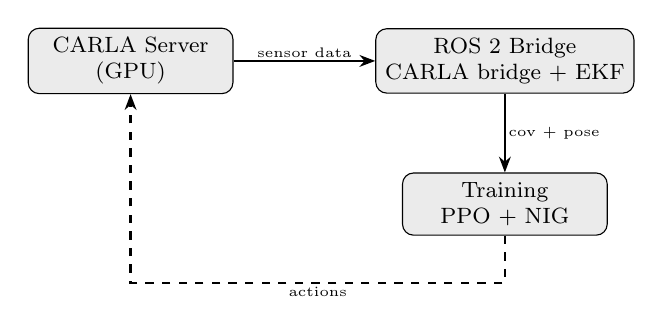
\begin{tikzpicture}[
    node distance=0.6cm and 0.4cm,
    box/.style={draw, rounded corners, minimum width=2.6cm, minimum height=0.7cm, font=\footnotesize, align=center},
    arrow/.style={-{Stealth[length=2mm]}, thick},
    lbl/.style={font=\tiny, midway, fill=white, inner sep=1pt}
]
\node[box, fill=black!8] (carla) {CARLA Server\\(GPU)};
\node[box, fill=black!8, right=1.8cm of carla] (ros) {ROS~2 Bridge\\CARLA bridge + EKF};
\node[box, fill=black!8, below=1.0cm of ros] (train) {Training\\PPO + NIG};
\draw[arrow] (carla) -- node[lbl,above] {sensor data} (ros);
\draw[arrow] (ros) -- node[lbl,right] {cov + pose} (train);
\draw[arrow, dashed] (train.south) -- ++(0,-0.6) -| node[lbl, below, pos=0.25] {actions} (carla.south);
\end{tikzpicture}}%
\caption{Three-container Docker architecture.\label{fig:architecture}}
\end{figure}

% To avoid having a policy which overfits to fixed spatial configurations, training episodes use a set of pre-computed parking lot floor plans defined in YAML layout files. Additional layouts can be produced on demand for out-of-distribution (OOD) evaluation while bay occupancy and dynamic actor placement are randomised per episode. Throughout training, periodic checkpoints are saved, and specific assessment containers provide replay using a windowed CARLA instance or a 2D bird's-eye visualiser.

\subsection{Layout Generation and Inspection}

Layout modules, each of which specifies a floor plan shape in a local coordinate frame, define the geometry of parking lots. Three shapes have been implemented: a $60 \times 45$\,m axis-aligned rectangle, a trapezium (front width 48\,m, rear width 30\,m, length 44\,m), and a nine-sided irregular polygon. The rectangle and trapezium will be used for training while the irregular polygon is reserved for out-of-distribution (OOD) evaluation to assess whether epistemic uncertainty increases. Further layouts can be added via the same interface.

Each module specifies spawn locations, patrol waypoints, pedestrian zone boundaries, perimeter cone positions interpolated along the polygon edges, and bay positions (perpendicular, angled, and parallel types according to the dimensional standards of the German parking design guideline EAR~05~\cite{fgsv2005ear}). An orchestrator script then applies a world-frame transform, producing bird's-eye PNG plots for visual verification (\cref{fig:rectangle}) as well as YAML layout files used by the training environment.

\begin{figure}[htbp]
    \centering
    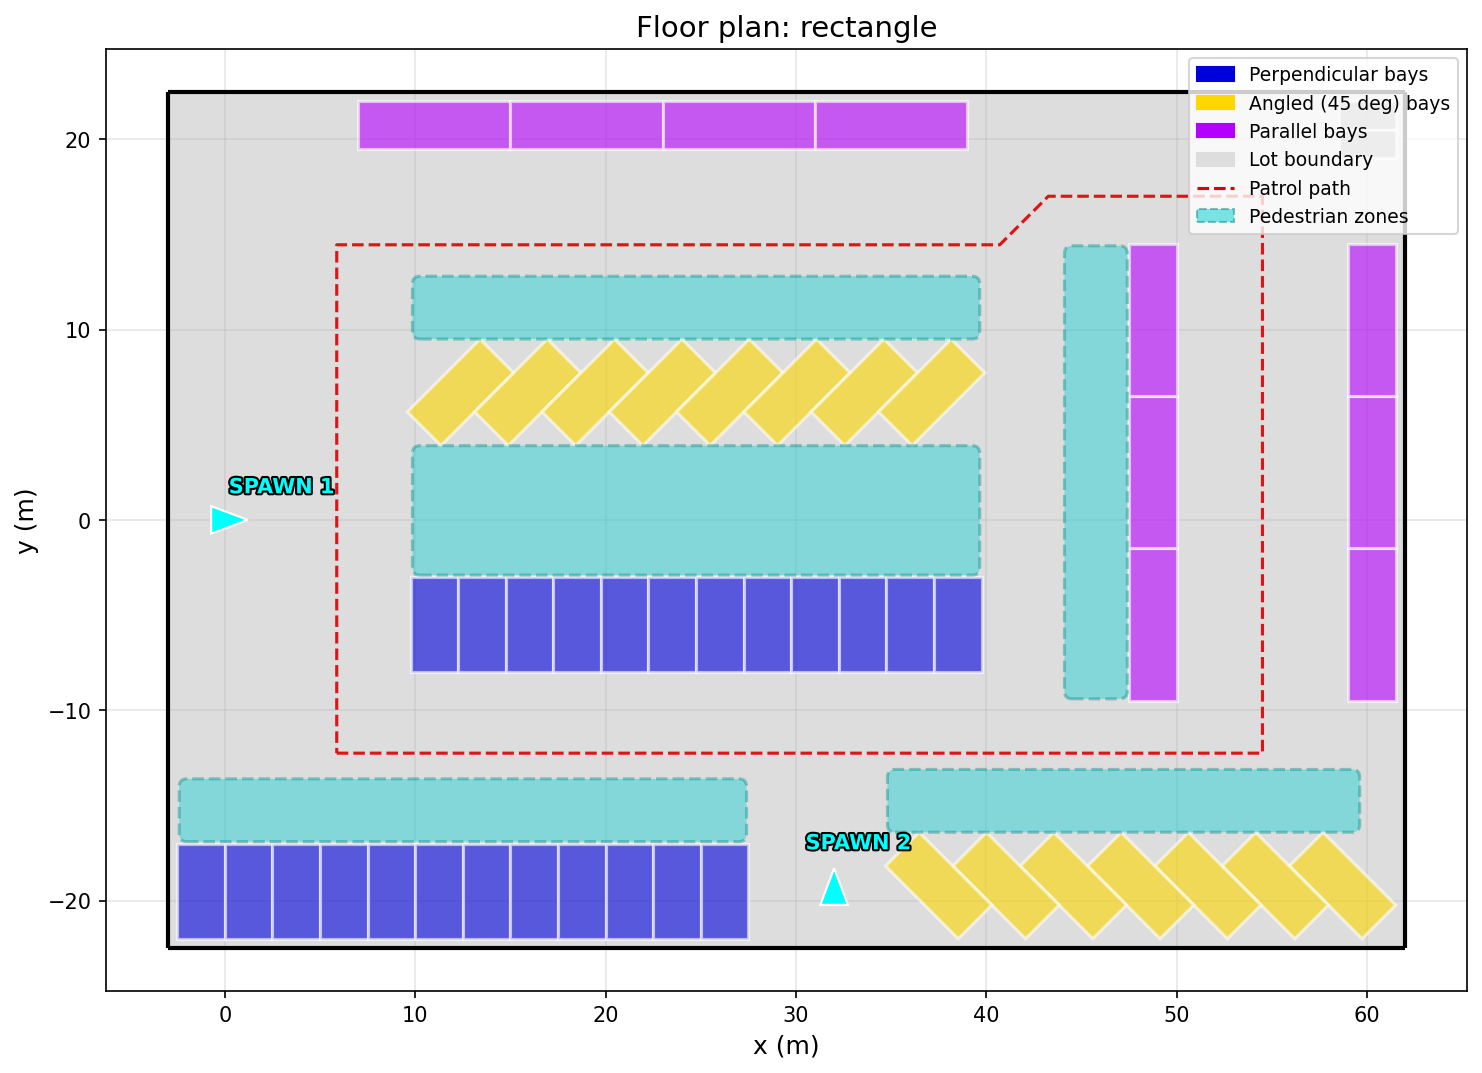
\includegraphics[width=\linewidth]{rectangle.png}
    \caption{Generated bird's-eye view of the rectangle floor plan showing bay positions (colour-coded by type), spawn points, patrol path and pedestrian zones.\label{fig:rectangle}}
\end{figure}

A unified inspector script provides four options for evaluating the system prior to training, all of which run inside dedicated Docker containers. In layout mode, the entire parking lot is created in windowed CARLA with geometry overlays presented as persistent debug primitives: spawn points, pedestrian zone boundaries, the patrol waypoint path, target bay highlighted in green, and bay outlines colour-coded by type. In sensors mode, the ego vehicle is spawned with each sensor mount point specified by a coloured dot, as illustrated in \cref{fig:sensors}, and the 2D LiDAR is also annotated with a field-of-view arc. In live mode, the obstacle detection range is visualised by rendering the 2D LiDAR scan returns as debug dots in the CARLA world. Lastly, dryrun mode allows the EKF localisation pipeline and observation construction to be tested end-to-end before any training is undertaken by running the whole training pipeline in windowed CARLA without a trained model, driven via teleoperation using a keyboard. In order to confirm that covariance inflates correctly with signal deterioration, root mean square error is calculated for position and heading and EKF pose predictions are compared to CARLA ground truth under each GNSS tier.

\begin{figure}[htbp]
    \centering
    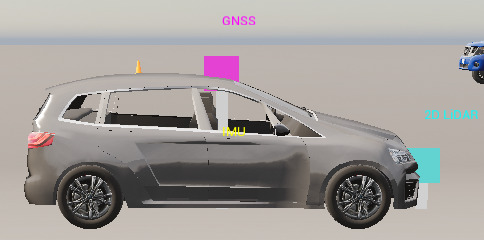
\includegraphics[width=\linewidth]{sensors.jpeg}
    \caption{Sensor inspector side-profile view indicating IMU, GNSS antenna and 2D LiDAR mount positions on the vehicle body.\label{fig:sensors}}
\end{figure}

On the other hand, a 2D bird's-eye visualiser is also implemented to evaluate the system during training. This works by using Pygame to render lot boundaries, bay outlines, NPC placements, and the ego vehicle trajectory trail by following a per-step log file written by the training environment (\cref{fig:visualiser}). To avoid additional overhead during training, a signal file is attached and detached to the visualiser at runtime, allowing evaluation to be performed without having to restart training. Furthermore, a 3D spectator mode offers a qualitative perspective on learnt driving behaviour by loading a saved checkpoint and replaying evaluation episodes in windowed CARLA. 

\begin{figure}[t]
    \centering
    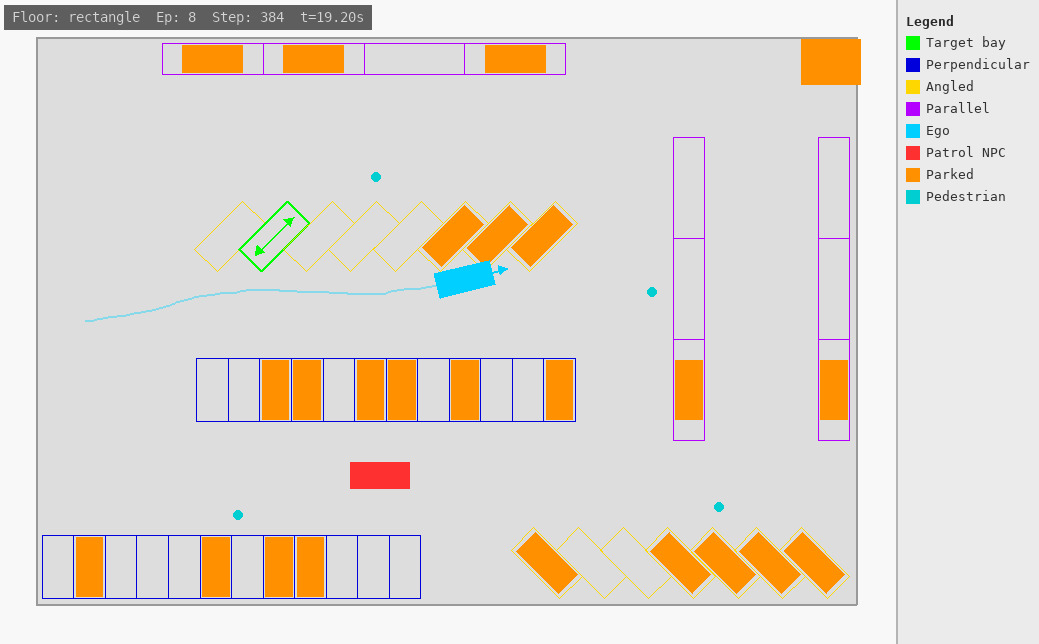
\includegraphics[width=\linewidth]{training.jpeg}
    \caption{Live bird's-eye training visualiser showing ego trajectory, bay outlines and NPC vehicles.\label{fig:visualiser}}
\end{figure}

\subsection{Observation Space}

The observation vector has 17 dimensions divided into four semantic groups, summarised in~\cref{tab:obs_space}. EKF velocity supplies the motion state for deceleration and alignment, the EKF covariance group exposes posterior uncertainty so the policy can condition on localisation confidence, and the relative target $(dx, dy, d\psi)$ encodes navigational intent in the ego body frame.

\begin{table}[htbp]
    \centering
    \caption{Observation space structure (17 dimensions).\label{tab:obs_space}}
    \begin{tabular}{lll}
        \toprule
        \textbf{Indices} & \textbf{Features} & \textbf{Source} \\
        \midrule
        0-2   & $v_x, v_y, \dot{\psi}$ & EKF velocity \\
        3-5   & $\sqrt{P_{xx}}, \sqrt{P_{yy}}, \sqrt{P_{\psi\psi}}$ & EKF std.\ devs \\
        6-8   & $P_{xy}, P_{x\psi}, P_{y\psi}$ & EKF cross-cov \\
        9-11  & $dx, dy, d\psi$ & Relative target \\
        12-16 & left/right/fwd clearance & 2D LiDAR \\
        \bottomrule
    \end{tabular}
\end{table}

The fourth group, hemispheric LiDAR clearance, provides five features from a single-plane 2D LiDAR~\cite{sick2026tim571}. The left and right hemispheres each contribute a nearest-obstacle distance and bearing, and the forward arc contributes distance alone given that its narrow 30-degree cone renders bearing redundant. The sensor is mounted at front-bumper height (0.5\,m above ground) so that the scan plane resolves perimeter cones, parked vehicles and pedestrians at heights characteristic of a parking environment.

The six covariance features comprise the three marginal standard deviations $\sqrt{P_{ii}}$ and the three off-diagonal cross-covariance terms $P_{xy}$, $P_{x\psi}$ and $P_{y\psi}$. The standard deviations provide a direct, interpretable measure of position and heading uncertainty in physical units, whilst the cross-covariance terms encode directional correlations between position and heading uncertainty that cannot be recovered from the marginal statistics alone. A signed log1p transformation, $\mathrm{sign}(x)\log(1+|x|)$, is applied to all six features to compress heavy tails whilst preserving the sign of off-diagonal terms. CARLA ground truth is only employed for reward computation and never appears in the observation, ensuring the policy does not rely on simulator state.

\subsection{Action Space}

The action space is two-dimensional and continuous. The first dimension is steering, $\delta \in [-1, 1]$, varying continuously across that range. The second dimension is a signed longitudinal command, $u \in [-1, 1]$, where positive values correspond to throttle and negative values to braking, with the environment decomposing this signal into separate CARLA throttle and brake actuator inputs at runtime. 

% \subsection{Two-Layer Uncertainty Architecture}

% The proposed architecture combines two complementary uncertainty mechanisms, illustrated in~\cref{fig:twolayer}. The input layer, consisting of EKF covariance elements in the observation vector, captures the confidence of the localisation system. The output layer, consisting of evidential NIG parameters on the actor, decomposes policy confidence into epistemic and aleatoric uncertainty, which can be used respectively to detect out-of-distribution situations and to quantify irreducible action ambiguity. Each layer responds to a distinct failure mode: degraded GNSS raises input uncertainty, whilst unfamiliar lot geometry raises output epistemic uncertainty. Their combination enables graduated responses ranging from cautious driving to full safety handoff.

% \begin{figure}[htbp]
% \centering
% \resizebox{\linewidth}{!}{%
% \begin{tikzpicture}[
%     node distance=0.6cm,
%     block/.style={draw, rounded corners, minimum width=2.6cm, minimum height=0.7cm, font=\footnotesize, align=center},
%     arrow/.style={-{Stealth[length=2mm]}, thick},
% ]
% % Centre actor block (reference point)
% \node[block, fill=black!12] (actor) {Evidential\\Actor (NIG)};

% % Left blocks - equidistant from actor centre line
% \node[block, fill=black!5, left=1.4cm of actor, yshift=0.7cm] (ekf) {EKF Covariance\\(6 dims)};
% \node[block, fill=black!5, left=1.4cm of actor, yshift=-0.7cm] (state) {Vehicle State\\+ Target Pose};

% % Right output block
% \node[block, fill=black!5, right=1.0cm of actor] (out) {$\gamma, \nu, \alpha, \beta$\\per action};

% % Arrow: EKF goes right then 90-deg down into actor.north
% \draw[arrow] (ekf.east) -- ++(0.45,0) |- (actor.170);

% % Arrow: State goes right then 90-deg up into actor.south
% \draw[arrow] (state.east) -- ++(0.45,0) |- (actor.190);

% % Actor -> output
% \draw[arrow] (actor.east) -- (out.west);

% % Labels
% \node[font=\tiny, above=0.15cm of ekf] {Layer 1: Input uncertainty};
% \node[font=\tiny, above=0.15cm of out] {Layer 2: Output uncertainty};
% \end{tikzpicture}}%
% \caption{Two-layer uncertainty architecture.\label{fig:twolayer}}
% \end{figure}

\subsection{Evidential Actor Head}

The actor's final layer produces NIG parameters $(\gamma, \nu, \alpha, \beta)$ per action dimension, with $\gamma$ serving as the predictive mean for action sampling, $a \sim \mathcal{N}(\gamma, \sigma^2_{\text{alea}})$. Positivity is enforced through the softplus function, $\text{softplus}(x) = \log(1 + e^x)$, with offsets:

\begin{align}
    \nu &= \text{softplus}(z_\nu) + \epsilon \nonumber \\
    \alpha &= \text{softplus}(z_\alpha) + 1 \nonumber \\
    \beta &= \text{softplus}(z_\beta) + \epsilon
    \label{eq:nig_constraints}
\end{align}

\noindent where $z_\nu$, $z_\alpha$ and $z_\beta$ are the raw pre-activation outputs of the final network layer and $\epsilon = 10^{-6}$. The unit offset on $\alpha$ ensures finite variance in~\cref{eq:nig_uncertainty}, with all three parameters additionally clamped to a maximum of 100 to prevent divergence in the RL setting, where no ground-truth action target exists. To prevent the NIG parameters from drifting arbitrarily far from their initialisations, a prior-anchoring log-penalty is applied:

\begin{equation}
    \mathcal{L}_{\text{reg}} = \lambda \left[ \overline{\log\!\left(\frac{\nu}{\nu_0} + 1\right)} + \overline{\log\!\left(\frac{\alpha}{\alpha_0} + 1\right)} \right]
    \label{eq:reg_loss}
\end{equation}

\noindent where $\nu_0, \alpha_0$ are initialisation-time values, $\lambda$ is linearly annealed from zero over a warmup period and $\overline{(\cdot)}$ denotes the mean over the batch and action dimensions. In contrast to the supervised regression regulariser of Amini et al.~\cite{amini2020deep}, this formulation is tailored for the RL situation, where $|a - \gamma|$ represents the intrinsic stochasticity of the policy instead of a prediction error against a known goal. These elements come together to form a single minimisation aim, and since $L^{\text{CLIP}}$ was specified as a quantity to be maximised, adding it to the total loss negates it:

\begin{equation}
    L = -L^{\text{CLIP}} + c_v L^{\text{VF}} - c_H H(\pi_\theta) + \mathcal{L}_{\text{reg}},
    \label{eq:total_loss}
\end{equation}

\noindent where $L^{\text{CLIP}}$ is the clipped surrogate objective from~\cref{eq:ppo}, $L^{\text{VF}}$ is the value function loss from~\cref{eq:vf_loss}, $c_v$ is the value function coefficient, $H(\pi_\theta)$ is the policy entropy, $c_H$ is its coefficient and $\mathcal{L}_{\text{reg}}$ is the evidential regularisation term from~\cref{eq:reg_loss}.

The training loop implementing the total loss from~\cref{eq:total_loss} is presented in~\cref{alg:training}. The NIG parameters $(\gamma, \nu, \alpha, \beta)$ are produced by the actor's forward pass during action evaluation within each mini-batch step and are then cached so that $\mathcal{L}_{\text{reg}}$ can be computed without a redundant forward pass. 
\begin{algorithm}[htbp]
    \caption{Evidential PPO training loop.\label{alg:training}}
    \begin{algorithmic}[1]
        \State Load configuration from YAML
        \State Initialise CARLA environment with EKF pipeline
        \State Normalise observations via running statistics
        \State Initialise EvidentialPPO with NIG actor head
        \For{each rollout of $n$ environment steps}
            \State Collect transitions $(s_t, a_t, r_t, s_{t+1})$
            \State Compute advantages via GAE
            \For{each optimisation epoch}
                \State Sample mini-batch
                \State Evaluate actions and cache NIG parameters 
                \State Compute $L^{\text{CLIP}}$, $L^{\text{VF}}$, $H(\pi_\theta)$ and $\mathcal{L}_{\text{reg}}$
                \If{approximate KL between $\pi_{\theta_{\text{old}}}$ and $\pi_\theta$ over the rollout exceeds $\text{KL}_{\text{target}}$}
                    \State Early-stop epoch loop
                \EndIf
                \State Backpropagate $L$ and update $\theta$
            \EndFor
            \State Log uncertainty metrics to TensorBoard
        \EndFor
        \State Save final model and normalisation statistics
    \end{algorithmic}
\end{algorithm}

% A dual-encoder variant of the actor processes vehicle state features and covariance features through separate encoder pathways before merging via concatenation into a shared trunk. This architectural separation permits the covariance pathway to develop specialised representations for uncertainty-dependent behaviour modulation.

\subsection{Hyperparameter Tuning}

Prior to the ablation study, Optuna is used to determine all hyperparameter values using a multivariate Tree-structured Parzen Estimator (TPE) sampler that models parameter interactions by estimating the joint density of high-performing configurations rather than treating each hyperparameter  independently~\cite{akiba2019optuna}. The search takes into account eight parameters: the learning rate, rollout length, mini-batch size, number of gradient epochs, entropy coefficient, evidential regularisation coefficient~$\lambda$, discount factor~$\gamma$, and its linear warmup time. The clipping range, gradient norm limit, KL target, and network architecture are held fixed, as large-scale sensitivity studies have identified these as low-variance dimensions across continuous control tasks~\cite{andrychowicz2021onpolicy}.

The study will run 35 trials, each training for 100{,}000 steps and evaluated on mean episodic progress reward, which provides a dense signal even when the agent infrequently achieves a successful park. Unpromising trials are terminated early by a MedianPruner~\cite{eimer2023hyperparams}. The best configuration is subsequently written to the training configuration file and applied without modification across all four ablation baselines.

% \subsection{Localisation Strategy}

% Scan-matching localisation against perimeter cones using Google Cartographer~\cite{hess2016cartographer} was initially evaluated as the primary localisation source. This approach was abandoned because parked vehicles occlude the cones when bay occupancy is high, causing localisation to degrade in precisely the conditions where reliable operation is most needed. Wheel odometry was similarly rejected because the simulator provides zero-noise ground truth, which suppresses the covariance variation that the policy must learn to interpret. RTK-GNSS was therefore adopted, providing well-characterised degradation modes from centimetre-level accuracy (RTK fixed) through metre-level (standalone). This choice restricts the system to outdoor parking lots with sky visibility, which is acknowledged as a scope limitation in~\cref{sec:evaluation}.

\subsection{GNSS Noise Model}

RTK-GNSS localisation quality is characterised as four discrete tiers, namely RTK fixed ($\sim$2\,cm), RTK float ($\sim$30\,cm), standalone ($\sim$2\,m) and degraded ($\sim$5\,m). Transitions between adjacent tiers are governed by a discrete-time Markov chain evaluated at the 20 Hz GNSS publishing rate, simulating gradual real-world variations in signal quality. These dynamics are encoded by the following transition probability matrix:

\begin{equation}
    \mathbf{T} = \begin{bmatrix}
        0.995 & 0.005 & 0     & 0     \\
        0.003 & 0.992 & 0.005 & 0     \\
        0     & 0.004 & 0.993 & 0.003 \\
        0     & 0     & 0.005 & 0.995
    \end{bmatrix}
    \label{eq:markov}
\end{equation}

\noindent where $T_{ij}$ denotes the probability of moving from tier $i$ to tier $j$ at the next time step, and transitions between non-adjacent tiers are forbidden. The high diagonal values ensure gradual rather than abrupt degradation, producing realistic mid-episode signal quality changes. These probabilities are deliberately chosen to over-represent degraded conditions during training, yielding a stationary distribution that places approximately 55\% of simulation time in standalone or degraded modes; this ensures sufficient exposure to rare failure modes rather than serving as a literal model of RTK availability in unobstructed outdoor environments. Furthermore, realistic IMU process noise derived from the VectorNav VN-100 datasheet~\cite{vectornav2023vn100} is additionally configured in the EKF to ensure covariance inflates appropriately between GNSS fixes. Both noise sources will assess the policy's ability to condition on localisation uncertainty.

\subsection{Reward Function}

The initial reward function employs distance-based shaping inspired by potential-based shaping~\cite{ng1999reward} to guide the agent toward the target bay:

\begin{equation}
    r_t = \frac{d_{t-1} - d_t}{d_{\max}} - c_{\text{step}},
    \label{eq:reward}
\end{equation}

\noindent where $d_t$ is the Euclidean distance to the target bay at step $t$, $d_{\max}$ is a fixed normalisation constant set to the approximate diagonal of the largest training lot and $c_{\text{step}}$ is a small per-step penalty. The formulation adapts the standard potential-based framework~\cite{ng1999reward} by replacing a state-dependent potential denominator with a fixed scale factor suited to the CARLA simulator. Beyond the dense per-step shaping signal, terminal rewards of $+10$ and $-10$ are awarded for success and collision respectively, where success requires position error $< 0.5$\,m, orientation error $< 10^\circ$ and speed $< 0.1$\,m/s simultaneously. 

\subsection{Dynamic Actors and Training Diversity}

To avoid the policy memorising a single static configuration, dynamic actors are added to each training episode. A single NPC patrol vehicle follows waypoint loops through the lot aisles via a proportional heading controller, braking when another actor is detected within a configurable forward-cone stop distance.

Within each designated pedestrian zone, a single pedestrian executes random walks and may be spawned with a configurable probability per episode, with zone confinement and ego-avoidance logic ensuring that any collision is only attributable to the ego vehicle. 

The target bay is always maintained empty and bay occupancy is randomised per episode. For perpendicular and angled target bays, neighbouring bays may be occupied, whereas for parallel bays they are kept vacant, as the agent lacks reverse functionality and forward-only entry requires lateral clearance. Finally, traffic cones are spaced consistently around the perimeter of the lot, and collisions with these result in episode termination with a collision penalty.

\newpage

\section{Evaluation Plan}
\label{sec:evaluation}

To separate the contribution of each uncertainty layer, a $2 \times 2$ factorial ablation study will be carried out, as detailed in~\cref{tab:ablation}. All four configurations will share identical PPO hyperparameters and each will be trained across three random seeds to assess seed-to-seed variability. A deterministic policy is evaluated over 100 episodes per condition, with GNSS and IMU noise multipliers, dynamic actor density, and bay occupancy held fixed.

\begin{table}[htbp]
    \centering
    \caption{Ablation study design.\label{tab:ablation}}
    \begin{tabular}{l|cc}
        \toprule
         & No EKF cov.\ (11d) & EKF cov.\ (17d) \\
        \midrule
        Standard actor & \texttt{vanilla\_ppo} & \texttt{input\_unc} \\
        Evidential actor & \texttt{output\_unc} & \texttt{full\_method} \\
        \bottomrule
    \end{tabular}
\end{table}

% The ablation cells correspond to the closest approaches in the literature. The \texttt{input\_unc} configuration, which feeds localisation uncertainty to a standard actor, is analogous to the approach of Puthumanaillam et al.~\cite{puthumanaillam2025guided}. The \texttt{output\_unc} configuration, which places an evidential head on the actor without covariance input, mirrors the evidential-in-RL strategy of Akg\"{u}l et al.~\cite{akgul2025eppo}, transposed from critic to actor. The \texttt{full\_method} configuration combines both layers and has no direct counterpart in existing work.

The following metrics are planned, each averaged across seeds and reported with standard deviation:

\begin{enumerate}

    \item \textbf{Success rate per GNSS tier.} A parking attempt will be defined as successful when the agent comes to rest within 0.5\,m of the target bay centre, within $10^\circ$ of the target heading and below 0.1\,m/s, with all three criteria met simultaneously. Success rate will be computed as the fraction of episodes satisfying these criteria, reported per ablation cell across the four GNSS tiers (RTK fixed, RTK float, standalone and degraded).

    \item \textbf{Collision rate under degraded GNSS.} The fraction of episodes in which a collision is registered by the CARLA physics engine under standalone (${\sim}2$\,m) and degraded (${\sim}5$\,m) noise conditions. This will be recorded for each ablation cell and compared across the $2 \times 2$ grid, following offline evaluation practices for driving models~\cite{codevilla2018offline}.

    \item \textbf{Graceful degradation curve.} Success rate will be plotted against GNSS noise multiplier for each ablation cell, producing a degradation profile for comparison across configurations.

    \item \textbf{Epistemic uncertainty on unseen layouts.} Mean per-step epistemic uncertainty on a held-out floor plan will be compared against the same configurations on a training layout under identical GNSS conditions, to assess whether the evidential head produces different uncertainty levels on novel geometry.

    \item \textbf{Aleatoric uncertainty across GNSS tiers.} Mean per-step aleatoric uncertainty will be recorded at each GNSS tier to investigate whether the policy learns to express higher action-level aleatoric noise when localisation quality degrades.

\end{enumerate}

% \section{Known Limitations and Future Directions}

% Several scope boundaries have been identified. The GNSS noise model currently applies isotropic diagonal covariance to the \texttt{NavSatFix} message; in practice, satellite geometry and multipath effects produce anisotropic error ellipses that vary with the vehicle's position relative to surrounding structures, and extending the model to incorporate directional covariance profiles is being considered.

% The Markov chain transition matrix governing GNSS fix-state changes is hand-tuned to approximate physically plausible dwell times; refining these probabilities based on empirical data could improve training fidelity. As noted in~\cref{sec:solution}, the adoption of RTK-GNSS restricts the system to outdoor parking lots with sky visibility; indoor or covered environments would require a different localisation source, though the uncertainty-conditioned policy architecture itself would transfer without modification. These boundaries do not affect the validity of the proposed architecture but represent directions along which the work could be extended.

\section{Conclusion}
\label{sec:conclusion}

The core system infrastructure has been completed: the RTK-GNSS localisation pipeline, CARLA simulation environment, GNSS Markov noise model, evidential PPO agent, and supporting inspection and visualisation tooling are all in place. Each uncertainty layer is independently exercisable through the ablation design, and the controlled GNSS degradation conditions are established. The end-to-end pipeline is undergoing final integration testing, after which hyperparameter optimisation will commence, followed by the full ablation study.

% \section*{Acknowledgments}
% This work is supervised by Dr Josef Bajada at the University of Malta, whose guidance has been invaluable throughout the research. I would also like to thank my company Lemonworx Ltd, especially Dr Graham Hili for his expertise and mentorship.

\newpage
{\small
\vspace*{-20pt}
\bibliographystyle{unsrt}
\bibliography{sigproc}
}

\newpage
\begin{figure*}[htbp]
\centering
\resizebox{\textwidth}{!}{%
\begin{ganttchart}[
    hgrid,
    vgrid={*{3}{draw=none}, dotted},
    x unit=0.65cm,
    y unit chart=0.55cm,
    title height=1,
    bar height=0.6,
    bar/.append style={fill=black!25},
    milestone/.append style={fill=black},
    group/.append style={fill=black!15},
    title label font=\footnotesize,
    bar label font=\footnotesize,
    group label font=\footnotesize\bfseries,
]{1}{24}
    \gantttitle{Apr}{4}
    \gantttitle{May}{4}
    \gantttitle{Jun}{4}
    \gantttitle{Jul}{4}
    \gantttitle{Aug}{4}
    \gantttitle{Sep}{4} \\

    \ganttgroup{Environment}{1}{6} \\
    \ganttbar{Integration testing}{1}{3} \\
    \ganttbar{Configuration tuning}{3}{6} \\

    \ganttgroup{Training}{5}{16} \\
    \ganttbar{Hyperparameter tuning}{5}{8} \\
    \ganttbar{Baseline (vanilla PPO)}{7}{10} \\
    \ganttbar{Input uncertainty}{9}{12} \\
    \ganttbar{Output uncertainty}{11}{14} \\
    \ganttbar{Full method}{13}{16} \\

    \ganttgroup{Evaluation}{13}{20} \\
    \ganttbar{Ablation analysis}{13}{16} \\
    \ganttbar{OOD / calibration tests}{15}{18} \\
    \ganttbar{Degradation curves}{17}{20} \\

    \ganttgroup{Dissertation}{9}{24} \\
    \ganttbar{Background \& Literature Review}{9}{12} \\
    \ganttbar{Design / implementation}{11}{16} \\
    \ganttbar{Results / evaluation}{17}{20} \\
    \ganttbar{Introduction / conclusion}{19}{22} \\
    \ganttbar{Review and corrections}{21}{24} \\

    \ganttmilestone{Submission}{24}

\end{ganttchart}
}
\caption{Dissertation work plan (April-September 2026).\label{fig:gantt}}
\end{figure*}

\balancecolumns
\end{document}